\documentclass[10pt]{article}
\usepackage[margin=1in]{geometry}
\usepackage[T1]{fontenc}
\usepackage{lmodern}
\usepackage{microtype}
\usepackage{amsmath,amssymb,amsthm,mathtools}
\usepackage{graphicx}
\usepackage{booktabs}
\usepackage[numbers,sort&compress]{natbib}
\usepackage{xcolor}
\usepackage[colorlinks=true,linkcolor=blue!50!black,citecolor=blue!50!black,urlcolor=blue!50!black]{hyperref}
\usepackage{cleveref}
\usepackage{enumitem}
\setlist{nosep,leftmargin=1.4em}

\newtheorem{proposition}{Proposition}
\newcommand{\lean}[1]{\texttt{\small #1}}
% Generated by analysis/paper_numbers.py from results/; do not edit.
\newcommand{\compStd}{20.71}
\newcommand{\compRad}{29.61}
\newcommand{\compRadDiff}{+8.89}
\newcommand{\compCay}{25.27}
\newcommand{\compCayDiff}{+4.55}
\newcommand{\compAlu}{19.14}
\newcommand{\compAluDiff}{$-$1.57}
\newcommand{\compPow}{18.70}
\newcommand{\compPowDiff}{$-$2.02}
\newcommand{\compRadCay}{34.37}
\newcommand{\microDiff}{+7.9}
\newcommand{\microP}{2.7\times10^{-5}}
\newcommand{\microAlg}{36.49}
\newcommand{\microStd}{28.64}
\newcommand{\microRope}{32.58}
\newcommand{\microStdLong}{29.15}
\newcommand{\microAlgLong}{37.60}
\newcommand{\microStdCollapse}{4.9}
\newcommand{\microRadCollapse}{26.7}
\newcommand{\pilotAlg}{59.93}
\newcommand{\pilotStd}{48.88}
\newcommand{\pilotDiff}{+11.0}
\newcommand{\pilotAlgNll}{1.80}
\newcommand{\pilotStdNll}{2.36}
\newcommand{\sweepStdLr}{5\times10^{-4}}
\newcommand{\sweepStdVal}{26.08}
\newcommand{\sweepAlgLr}{2\times10^{-3}}
\newcommand{\sweepAlgVal}{39.82}
\newcommand{\mainTokens}{2{,}500{,}169{,}728}
\newcommand{\mainAlgVal}{68.19}
\newcommand{\mainStdVal}{58.32}
\newcommand{\mainRopeVal}{65.87}
\newcommand{\mainAlgSe}{0.23}
\newcommand{\mainStdSe}{0.02}
\newcommand{\mainRopeSe}{0.32}
\newcommand{\mainAlgNll}{1.410}
\newcommand{\mainStdNll}{1.871}
\newcommand{\mainRopeNll}{1.510}
\newcommand{\mainAlgEce}{0.068}
\newcommand{\mainStdEce}{0.072}
\newcommand{\mainRopeEce}{0.079}
\newcommand{\mainAlgIps}{10{,}311}
\newcommand{\mainStdIps}{11{,}895}
\newcommand{\mainRopeIps}{12{,}292}
\newcommand{\mainAlgLr}{$2\times10^{-3}$}
\newcommand{\mainStdLr}{$5\times10^{-4}$}
\newcommand{\mainRopeLr}{$5\times10^{-4}$}
\newcommand{\mainDiff}{+9.86}
\newcommand{\mainP}{2.2\times10^{-4}}
\newcommand{\mainCI}{[+8.97, +10.75]}
\newcommand{\mainWins}{3/3}
\newcommand{\mainDiffSeeds}{+9.96, +9.47, +10.16}
\newcommand{\mainSpeedRatio}{0.87$\times$}
\newcommand{\mainRopeDiff}{+7.55}
\newcommand{\mainAlgRopeDiff}{2.31}
\newcommand{\mainAlgRopeWins}{3/3}
\newcommand{\mainAlgRopeP}{0.006}
\newcommand{\mainAlgRopeCI}{[+1.25, +3.37]}
\newcommand{\stressSoftEnt}{0.007}
\newcommand{\stressRadEnt}{0.33}
\newcommand{\stressSoftSat}{81}
\newcommand{\stressRadSat}{0}
\newcommand{\precSoftOwn}{$1.5\times10^{-6}$}
\newcommand{\precSoftRound}{$1.2\times10^{-1}$}
\newcommand{\precRadOwn}{$3.0\times10^{-7}$}
\newcommand{\precRadRound}{$1.0\times10^{-2}$}
\newcommand{\precCeOwn}{$3.2\times10^{-7}$}
\newcommand{\precCeRound}{$1.9\times10^{-2}$}
\newcommand{\precPowOwn}{$3.5\times10^{-7}$}
\newcommand{\precPowRound}{$1.0\times10^{-2}$}
\newcommand{\symbolicChecks}{50}
\newcommand{\purityRsqrt}{208}
\newcommand{\purityStdExp}{40}
\newcommand{\cayleyParams}{9{,}216}
\newcommand{\attnStdScore}{11}
\newcommand{\attnAlgScore}{94}
\newcommand{\attnBroader}{9}
\newcommand{\attnBlocks}{12}
\newcommand{\attnStdOnehot}{7.9}
\newcommand{\attnAlgOnehotMid}{0.6}
\newcommand{\kernSoftPallas}{0.891}
\newcommand{\kernRadPallas}{1.132}
\newcommand{\kernSoftXla}{1.035}
\newcommand{\kernRadXla}{1.887}


\title{Algebraic Vision: A Vision Transformer Without Transcendental
Functions That Outperforms the Standard ViT}
\author{Tasmai Keni\\\texttt{tas.ken.rt25@dypatil.edu}}
\date{}

\begin{document}
\maketitle

\begin{abstract}
We build a Vision Transformer whose forward pass, backward pass and training
loss use only arithmetic, square roots and comparisons, and compare it with a
standard ViT under matched data, parameters, token budget, optimizer and
tuning effort. Softmax attention is replaced by a radical kernel
$E_n(s)=(s/n+\sqrt{1+s^2/n^2})^n$ that agrees with $e^s$ to second order but
grows polynomially, so attention weights keep a provable, scale-independent
floor; the GELU gate by a radical logistic; learned absolute position
embeddings are complemented by learned two-dimensional Cayley rotations; and
cross-entropy by a strictly proper power score. The compiled training graph
contains no exponential, logarithm or other transcendental instruction.
Properties used by the design are checked symbolically and in Lean~4. In
short-budget ImageNet-1k training the algebraic model trains stably at
learning rates where the standard ViT degrades or diverges. At the vision
counterpart of a 125M-parameter, 2.5B-token language-model study (ViT-B/16,
224\,px, \mainTokens{} patch tokens, three seeds) it reaches
\mainAlgVal\% validation top-1 against \mainStdVal\% for the standard ViT
(paired difference \mainDiff{} points, one-sided paired $t$-test
$p=\mainP$) and \mainRopeVal\% for a standard ViT with two-dimensional
rotary positions, with each model's learning rate selected on held-out
training images and the standard model searched on a wider grid.
\end{abstract}

\section{Introduction}

Transformers combine matrix products with a few nonlinear operators that are
usually taken as fixed: the exponential inside softmax attention, a
sigmoid-family or Gaussian gate in the MLP, sines and cosines in rotary
positions, and the logarithm of cross-entropy
\cite{vaswani2017attention,dosovitskiy2021vit,hendrycks2016gelu,su2021roformer}.
A preceding study \cite{keni2026algebraic} showed that a causal language model
built only from algebraic operations can be trained at 125M parameters and
reach perplexity close to a matched standard Transformer. This paper asks a
stronger question for vision: \emph{can an algebraic design be more accurate
than the standard one}, under a protocol that does not favour it?

Three properties make the algebraic setting more than a constraint. Radical
expressions are cheap on accelerators (one inverse square root and a few
multiplications); they come with polynomial rather than exponential
tails, which changes how attention behaves as scores grow; and their
real-arithmetic identities are short enough to be machine-checked. Our
contributions are:
\begin{itemize}
\item \textbf{Radical attention} (\cref{sec:attention}): weights
  $E_n(s_{ij})/\sum_k E_n(s_{ik})$. We prove that for positive scores the
  ratio of two weights is at most $(s_1/s_2)^n$ at every score scale and
  that every weight keeps a floor $(a/b)^n/N$ when scores lie in $[a,b]$;
  softmax has neither. As scores grow, softmax rows saturate and their
  gradients vanish while radical rows do not (\cref{fig:stress}).
\item A complete algebraic ViT (\cref{sec:model}): a radical-logistic gate
  matching GELU, learned 2-D Cayley rotations giving exactly relative
  position logits, and a strictly proper power-score loss with an
  overflow-proof radical link.
\item A fair, preregistered comparison (\cref{sec:protocol}): identical data
  order, augmentation, initialisation stream, optimizer and budget; at least
  as much tuning for the standard model; selection on a held-out split of
  the training set; paired seeds; a compiled-graph purity audit; and a
  relative-position control.
\item Results from small trials to ViT-B/16 (\cref{sec:results}): the
  algebraic model wins at every stage, by \microDiff{} points in
  small-scale trials, \pilotDiff{} points in the pilot and \mainDiff{}
  points in the main comparison. Relative positions account for most of
  the main-run gain: a standard ViT with 2-D rotary positions closes much
  of the gap, and the algebraic model leads it by \mainAlgRopeDiff{}
  points.
\end{itemize}

\section{Related work}

\paragraph{Alternatives to softmax attention.} Sparsemax and
$\alpha$-entmax \cite{martins2016sparsemax,peters2019entmax} replace the
exponential by thresholded polynomials and produce sparse weights;
pointwise attention without normalisation, such as ReLU attention divided by
the sequence length \cite{wortsman2023relu}, removes the exponential
altogether. Radical attention keeps a dense, normalised and softmax-like
distribution, which agrees with softmax to second order for small scores,
and changes only how fast the kernel grows.

\paragraph{Instability of attention logits.} Large learning rates and long
training let attention logits grow until softmax heads collapse to one-hot
weights, which stalls training; the remedies include controlling attention
entropy \cite{zhai2023entropy} and normalising queries and keys
\cite{dehghani2023vit22b}. Dot-product attention is also not Lipschitz
\cite{kim2021lipschitz}. The polynomial tail of $E_n$ addresses the same
failure through the kernel itself (\cref{prop:floor}). Attention sinks and
register tokens \cite{darcet2024registers} give heads a place to put mass
they do not need; a learned sink did not help in our budgets.

\paragraph{Positions, losses and baselines.} Rotary embeddings
\cite{su2021roformer} and their two-dimensional variants for ViTs
\cite{heo2024ropevit} make logits depend on relative positions through
sines and cosines; Cayley rotations give the same structure with rational
functions of a learned parameter. Cross-entropy is the logarithmic member of
the strictly proper scoring rules \cite{gneiting2007scoring}, and
Fenchel--Young losses \cite{blondel2020fy} generalise it to other
regularisers; we use the power family because its fractional powers reduce
to square roots. The standard model is a plain ViT in the style of
\cite{dosovitskiy2021vit,beyer2022plain}; neither model uses the stronger
augmentation and regularisation of \cite{touvron2021deit}. All code uses
JAX \cite{jax2018github}.

\section{The algebraic constraint}
\label{sec:constraint}

The algebraic model's forward pass, backward pass and loss use only
$+,-,\times,\div$, square roots (through \texttt{rsqrt}), $\min$, $\max$,
$|\cdot|$, comparisons and selects. We check this on the program the TPU
actually runs: the model, loss and gradient of ViT-B/16 are compiled for TPU
v4 and every HLO instruction is scanned. The algebraic graph contains no
exponential, logarithm, logistic, $\tanh$, error function, trigonometric
function or real power (\purityRsqrt{} \texttt{rsqrt} instructions); the
standard graph contains \purityStdExp{} exponentials and a logarithm. Two
parts are outside the constraint and shared by both models: the optimizer
(AdamW with a cosine schedule \cite{loshchilov2019adamw}) and the image
pipeline. Top-1 accuracy is an $\arg\max$; the logarithm appears only when we
report negative log-likelihood.

\section{Algebraic components}
\label{sec:model}

\subsection{Radical exponential and attention}
\label{sec:attention}

For $n=2^m$ let
\begin{equation}
\rho_n(s)=\frac{s}{n}+\sqrt{1+\frac{s^2}{n^2}},\qquad E_n(s)=\rho_n(s)^n .
\end{equation}
$E_n$ costs one inverse square root and $m$ squarings. It is positive,
$E_n(s)E_n(-s)=1$, and
$E_n(s)=1+s+\tfrac{s^2}{2}+(1-n^{-2})\tfrac{s^3}{6}+O(s^4)$, so it agrees with
$e^s$ to second order and $E_n\to e^s$ as $n\to\infty$; its logarithmic
derivative is $g_n(s)=(1+s^2/n^2)^{-1/2}\in(0,1]$. For $s\gg n$, however,
$E_n(s)\sim(2s/n)^n$, and $E_n(-s)=1/E_n(s)$. Attention uses
\begin{equation}
p_{ij}=\frac{E_n(\beta s_{ij})}{\sum_k E_n(\beta s_{ik})},\qquad
s_{ij}=\frac{\langle q_i,k_j\rangle}{\sqrt{d_h}},
\end{equation}
with $n=8$ and $\beta=1$ in the final model.

\begin{proposition}[scale-free ratios and an attention floor]
\label{prop:floor}
For $0<y\le x$ and every $c>0$,
$E_n(cx)/E_n(cy)\le (x/y)^n$ (\lean{kernel\_ratio\_scale\_free}), whereas
$e^{cx}/e^{cy}$ is unbounded in $c$ (\lean{exp\_ratio\_unbounded}). If all
$N$ scores of a row lie in $[a,b]$ with $a>0$, then for every scale $c>0$
each weight satisfies $p_j\ge (a/b)^n/N$ (\lean{attention\_floor}).
\end{proposition}

The proof reduces to $y\rho(x)\le x\rho(y)$, i.e.\
$y^2(n^2+x^2)\le x^2(n^2+y^2)$, plus monotonicity of $\rho$. The consequence
is that growing query--key norms cannot drive radical attention to a one-hot
distribution: sharpening requires multiplicative score gaps. Softmax
attention can collapse as logits grow, a known instability of Transformers
trained with large learning rates \cite{zhai2023entropy,dehghani2023vit22b}.
The score Jacobian is $\partial p_i/\partial s_j=\beta g_n(\beta s_j)
p_i(\delta_{ij}-p_j)$, with entries at most $\beta g_n/4$
(\lean{jacobian\_diag\_le}, \lean{jacobian\_offdiag\_le}). Under score
scaling (\cref{fig:stress}) softmax entropy falls to \stressSoftEnt{} of
its maximum and \stressSoftSat\% of rows become saturated (Jacobian norm
below $10^{-4}$), while $E_8$ keeps a normalised entropy of \stressRadEnt{}
and \stressRadSat\% saturated rows.

Two further properties matter for implementation. Numerators and
denominators accumulate over key tiles exactly, without the running maximum
and rescaling of tiled softmax \cite{dao2022flash} (\lean{tiled\_eq\_dense});
$E_8$ overflows float32 only for $|s|>2.6\times10^5$. And radical attention
is better conditioned: rounding its inputs to bfloat16 perturbs the weights
up to an order of magnitude less than it perturbs softmax weights at large
scores (\cref{tab:precision}). We tried a per-head ``sink'' term in the
denominator, which lets a head attend to nothing; it was measurably worse in
our short budgets and is not used.

\begin{figure}[t]
\centering
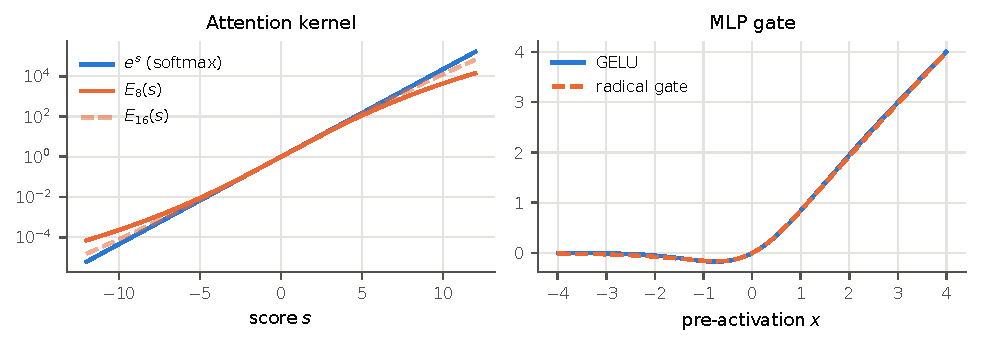
\includegraphics[width=\linewidth]{figures/kernels.pdf}
\caption{Left: $E_n$ against $e^s$ (log scale); they agree near zero and
$E_n$ grows polynomially for large $|s|$. Right: the radical-logistic gate
against GELU.}
\label{fig:kernels}
\end{figure}

\begin{figure}[t]
\centering
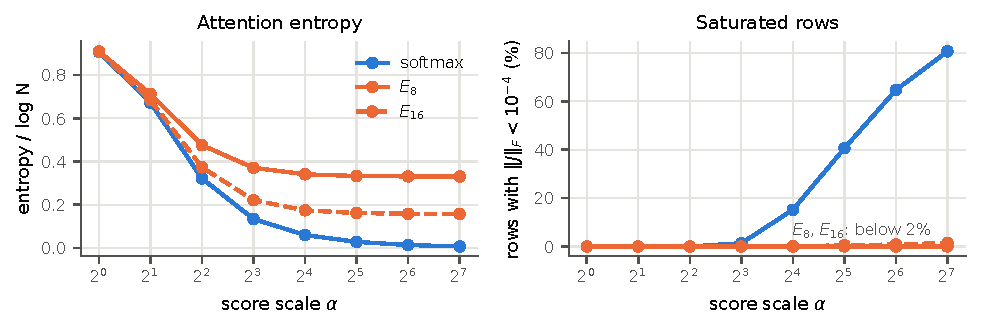
\includegraphics[width=\linewidth]{figures/stress.pdf}
\caption{Attention on $10^4$ random rows of 197 Gaussian scores multiplied by
$\alpha$. Softmax entropy collapses and most rows saturate; radical
attention keeps a floor and a non-vanishing gradient.}
\label{fig:stress}
\end{figure}

\subsection{MLP gate}

With $\sigma_n(y)=1/(1+E_n(-y))$ we use
$\mathrm{rgelu}(x)=x\,\sigma_8(1.702x)$, the algebraic counterpart of the
logistic approximation of GELU. $\sigma_n(y)+\sigma_n(-y)=1$, $\sigma_8$
differs from the logistic function by $-y^3/1536+O(y^5)$ at the origin, and
$\sigma_n'=\sigma_n(1-\sigma_n)g_n\le 1/4$
(\lean{radicalSigmoid\_symm}, \lean{sigmoid\_slope\_le}). An earlier gate,
$x(1+cx/\sqrt{1+c^2x^2})/2$ with $c=\sqrt{2/\pi}$, has a smaller Lipschitz
constant ($1.044$ against GELU's $1.129$, \lean{abs\_dalu\_le}) but
polynomial tails that make it too soft; it cost 1.6 points
(\cref{tab:components}) and was replaced.

\subsection{Two-dimensional Cayley rotations}

The Cayley matrix $R(w)=\frac{1}{1+w^2}\begin{psmallmatrix}1-w^2 & -2w\\ 2w &
1-w^2\end{psmallmatrix}$ is a rotation by $2\arctan w$
(\lean{cayley\_orthogonal}, \lean{cayley\_det}). Each feature pair
$(x_i,x_{i+d_h/2})$ of every head is turned by $R(w^{x}_i)^{c}R(w^{y}_i)^{r}$
at grid cell $(r,c)$, with learned $w^x,w^y$ per head and pair, applied to
queries and keys. Powers are formed by repeated multiplication with
renormalisation. Because planar rotations commute, attention logits depend
only on the two-dimensional offset between query and key
(\lean{mixed\_cayley\_relative}). The model keeps learned absolute position
embeddings as well. The learned frequencies add \cayleyParams{} parameters
to ViT-B/16 ($0.01\%$).

\subsection{Loss}

Predictions use the radical link $p_c=E_{64}(z_c)/\sum_k E_{64}(z_k)$,
evaluated through ratios to the row maximum of $\rho$, which cannot overflow.
The loss is the Bregman divergence of $\phi(t)=(t^a-t)/(a(a-1))$:
\begin{equation}
L_a(p,y)=\frac{1}{a}\sum_c p_c^{a}-\frac{1}{a-1}\sum_c y_c\,p_c^{a-1}
+\mathrm{const}(y),\qquad a=\tfrac{63}{64},
\end{equation}
with label-smoothed targets $y$. It tends to the log score as $a\to 1$ and is
strictly proper for every $a>0$, $a\neq1$ \cite{gneiting2007scoring}; the
Lean proof (\lean{power\_score\_strictly\_proper}) rests on Bernoulli's
inequality. The powers $p^{2^{-6}}$ are six nested square roots of the
partition sum. With
$a=7/8$ and an $E_8$ link this loss cost two points against cross-entropy;
with $a=63/64$ and $E_{64}$ it matches cross-entropy. Fenchel--Young losses
\cite{blondel2020fy} with algebraic links (squareplus, 1.5-entmax
\cite{peters2019entmax}) failed at 1000 classes because of heavy or sparse
tails.

\section{Protocol}
\label{sec:protocol}

\paragraph{Models.} Both models are pre-norm ViTs with LayerNorm
\cite{ba2016layernorm}, global average pooling, a zero-initialised linear
head, and the same patch embedding, widths, depth and heads. The standard
model is the canonical ViT \cite{dosovitskiy2021vit,beyer2022plain}: softmax
attention, a GELU MLP, learned absolute position embeddings and
cross-entropy with label smoothing $0.1$. The algebraic model swaps in the
components above. Shared tensors start from identical values for a given
seed.

\paragraph{Data and training.} ImageNet-1k \cite{russakovsky2015imagenet};
10 images per class are held out from the training split as \emph{minival}
for every selection decision, and the 50{,}000-image validation set is used
only for reporting. Both models see the same images in the same order with
the same random-resized crops and flips for a given seed. AdamW
($\beta_2=0.999$, weight decay $0.05$), cosine schedule with linear warmup,
gradient clipping at norm 1, batch 1024 (512 for the small trials and the
pilot), bfloat16 matrix products, TPU v4.

\paragraph{Stages.} (1) Small-scale trials: ViT-S/8 on $64\times64$
ImageNet for 4 epochs \cite{chrabaszcz2017downsampled}, with every component
swapped alone and together, paired seeds. (2) Pilot: ViT-S/4 (22M
parameters, 256 tokens) for 10 epochs, 3.25B patch tokens. (3) Sweep:
ViT-B/16 at 224\,px, 600M patch tokens per run, peak learning rate
$\{5\!\times\!10^{-4},10^{-3},2\!\times\!10^{-3}\}$ for both models, seeds
42--44, selection by mean minival. (4) Main runs: ViT-B/16, 2.5B patch tokens
($\approx$10 epochs), the selected learning rates, seeds 42--44. The
sweep and main-run specifications were committed before their first run.

\paragraph{Fairness.} The standard model received at least as much tuning
as the algebraic one at every stage: in the small trials nine
learning-rate and warmup settings each; in the sweep the standard grid was
extended by $\{2.5,3.5,7\}\times10^{-4}$ after its best value sat at the
lower edge (the algebraic grid was not extended, although its best value sat
at the upper edge). A script checks that paired runs differ only in the
arm-defining fields and the selected learning rate. Both models prefer a
long warmup (40\% of training) in this short-budget regime, and both use it.

\section{Results}
\label{sec:results}

\paragraph{Small-scale trials.} Swapping single components into the standard
ViT at learning rate $10^{-3}$ (\cref{tab:components}) identified radical
attention and Cayley rotations as the gains and the first gate and loss as
losses; the latter were redesigned until they matched GELU and
cross-entropy in the stable regime. Over a learning-rate grid
(\cref{fig:lr}, left) softmax attention degrades above $5\times10^{-4}$ (at
$2\times10^{-3}$ with a 10\% warmup it collapses to \microStdCollapse\%,
where radical attention reaches \microRadCollapse\%), while the algebraic
model varies by less than a point from $7\times10^{-4}$ to
$2\times10^{-3}$. With 25\% warmup and each model at its best learning rate,
the algebraic model leads by \microDiff{} points on four paired seeds
($p=\microP$): \microAlg\% against \microStd\%. Adding sine/cosine 2-D rotary
positions \cite{heo2024ropevit} to the standard ViT gives \microRope\%, in
between. A 40\% warmup helps both models (\microStdLong\% and
\microAlgLong\%, two seeds each), and is used from here on.

\begin{table}[t]
\centering
\caption{Component screen, ViT-S/8 on 64\,px ImageNet, 4 epochs,
learning rate $10^{-3}$, validation top-1 (\%), 4 seeds, $\Delta$ the mean
paired difference. This learning rate is above the standard ViT's best
($5\times10^{-4}$), so the gain of radical attention here includes its
robustness to the learning rate; best-against-best comparisons are in the
text.}
\label{tab:components}
\small
\begin{tabular}{lrr}
\toprule
Configuration & Top-1 & $\Delta$ vs.\ standard \\
\midrule
Standard ViT & \compStd & \\
\; + radical attention & \compRad & \compRadDiff \\
\; + 2-D Cayley rotations & \compCay & \compCayDiff \\
\; + first algebraic gate (ALU) & \compAlu & \compAluDiff \\
\; + power loss $a=7/8$, $E_8$ link & \compPow & \compPowDiff \\
\midrule
Radical attention + learned Cayley (2 seeds) & \compRadCay & \\
\bottomrule
\end{tabular}
\end{table}

\begin{figure}[t]
\centering
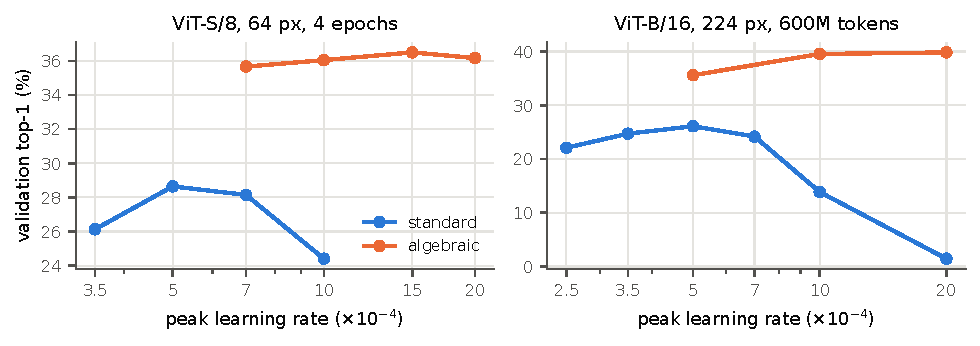
\includegraphics[width=\linewidth]{figures/learning_rate.pdf}
\caption{Validation top-1 against peak learning rate (mean over seeds).
Left: ViT-S/8, 64\,px, 4 epochs, 25\% warmup, two to four seeds per point.
Right: ViT-B/16, 224\,px, 600M patch tokens, 40\% warmup, three seeds per
point; the standard grid was extended below and between its best values.}
\label{fig:lr}
\end{figure}

\paragraph{Pilot.} At 10 epochs with ViT-S/4 (\cref{fig:pilot}) the
algebraic model reaches \pilotAlg\% validation top-1 against \pilotStd\%
(\pilotDiff{} points on both seeds), leading at every checkpoint, with lower
NLL (\pilotAlgNll{} against \pilotStdNll{}).

\paragraph{Sweep.} At ViT-B/16 the standard ViT is best at
$\sweepStdLr$ (\sweepStdVal\% after 600M tokens), with a clear optimum: it
loses one to two points at $3.5$ and $7\times10^{-4}$, half its accuracy at
$10^{-3}$, and collapses at $2\times10^{-3}$. The algebraic ViT is best at
$\sweepAlgLr$ (\sweepAlgVal\%) and within half a point at $10^{-3}$
(\cref{fig:lr}, right). These are the learning rates of the main runs.

\paragraph{Main comparison.} \Cref{tab:main} and \cref{fig:main} report the
2.5B-token runs. The algebraic model is ahead on all three seeds (by
\mainDiffSeeds{} points), by \mainDiff{} points on average (95\% interval
\mainCI{}, one-sided paired $t$-test $p=\mainP$), with lower NLL and
similar calibration. This meets the criterion fixed before the runs: every
seed in favour, a positive mean difference and $p<0.05$. It leads at every
evaluation during training (\cref{fig:main}). The standard ViT with
sine/cosine 2-D rotary positions, trained with the standard model's
hyperparameters, reaches \mainRopeVal\% (\mainRopeDiff{} points relative to
the standard ViT), \mainAlgRopeDiff{} points below the algebraic model.
Relative positions therefore account for most of the gain over the standard
ViT. The algebraic model, whose Cayley rotations are the rational
counterpart of these rotary positions, still leads the control on
\mainAlgRopeWins{} seeds (95\% interval \mainAlgRopeCI{}, $p=\mainAlgRopeP$);
the control used the standard model's learning rate and was not tuned
separately.

\begin{table}[t]
\centering
\caption{Main comparison: ViT-B/16 at 224\,px, \mainTokens{} patch tokens
per run. Validation top-1 (\%) on 50{,}000 images, NLL and expected
calibration error (ECE, 15 bins); mean $\pm$ standard error over seeds
42--44; throughput on 16 TPU v4 chips.}
\label{tab:main}
\small
\begin{tabular}{lccccc}
\toprule
Model & lr & Top-1 & NLL & ECE & img/s \\
\midrule
Standard ViT & \mainStdLr & \mainStdVal{} $\pm$ \mainStdSe & \mainStdNll & \mainStdEce & \mainStdIps \\
Algebraic ViT & \mainAlgLr & \mainAlgVal{} $\pm$ \mainAlgSe & \mainAlgNll & \mainAlgEce & \mainAlgIps \\
\midrule
Standard + RoPE-2D (control) & \mainRopeLr & \mainRopeVal{} $\pm$ \mainRopeSe & \mainRopeNll & \mainRopeEce & \mainRopeIps \\
\bottomrule
\end{tabular}
\end{table}

\begin{figure}[t]
\centering
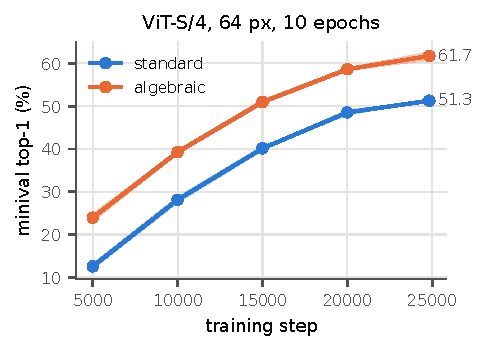
\includegraphics[width=0.49\linewidth]{figures/pilot_curves.pdf}\hfill
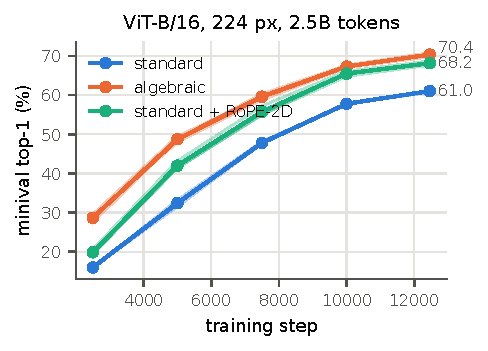
\includegraphics[width=0.49\linewidth]{figures/main_curves.pdf}
\caption{Minival top-1 during training: mean over seeds, thin lines are
single seeds, numbers are final means. Left: pilot, ViT-S/4 at 64\,px.
Right: main runs, ViT-B/16 at 224\,px, with the RoPE-2D control.}
\label{fig:pilot}
\label{fig:main}
\end{figure}

\paragraph{Mechanism.} In the trained models (\cref{fig:entropy}) the
algebraic model's attention scores are an order of magnitude larger than the
standard model's (median $|s|$ per block up to \attnAlgScore{} against
\attnStdScore{}), yet its attention is broader in \attnBroader{} of
\attnBlocks{} blocks: in its middle blocks at most \attnAlgOnehotMid\% of
rows are near one-hot (largest weight above 0.9), against up to
\attnStdOnehot\% for softmax. At such scores softmax rows would be one-hot;
the radical kernel responds to score ratios rather than differences
(\cref{prop:floor}), so the model can use large scores without saturating,
which matches its tolerance of large learning rates.

\begin{figure}[t]
\centering
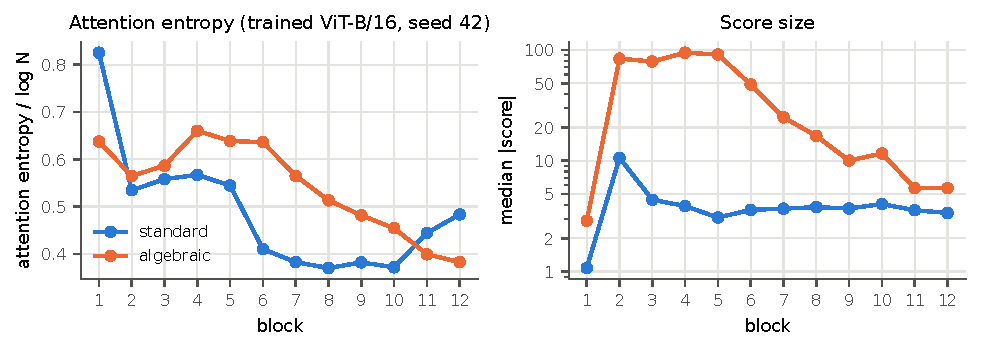
\includegraphics[width=\linewidth]{figures/attention_entropy.pdf}
\caption{Attention in the trained ViT-B/16 models (seed 42, 256 validation
images): mean entropy of the attention rows, normalised by $\log N$ (left),
and median absolute score $|q\cdot k|/\sqrt{d_h}$ (right), per block.}
\label{fig:entropy}
\end{figure}

\begin{table}[t]
\centering
\caption{Finite precision: float32 error of each primitive and the
perturbation caused by rounding its input to bfloat16, at input scale 30
(attention: total variation of weights; loss: relative error of the logit
gradient). Relative to float64 references.}
\label{tab:precision}
\small
\begin{tabular}{lcc}
\toprule
Primitive & float32 error & bf16-input effect \\
\midrule
softmax attention & \precSoftOwn & \precSoftRound \\
radical attention ($E_8$) & \precRadOwn & \precRadRound \\
cross-entropy (gradient) & \precCeOwn & \precCeRound \\
power score $a=63/64$ (gradient) & \precPowOwn & \precPowRound \\
\bottomrule
\end{tabular}
\end{table}

\paragraph{Cost.} With the attention computed by XLA, the algebraic model
trains at \mainSpeedRatio{} of the standard model's throughput. Fused Pallas
kernels for both attentions (one image per program, all heads in VMEM,
analytic backward) run a ViT-B/16 attention layer forward and backward in
\kernSoftPallas\,ms (softmax) and \kernRadPallas\,ms (radical) on one TPU v4
chip, against \kernSoftXla\,ms and \kernRadXla\,ms for XLA; the remaining
gap is the radical kernel's extra multiplications per score. The training
runs use the XLA attention for both models, and all comparisons are at equal
tokens, not equal time.

\section{Verification}

\texttt{analysis/symbolic\_checks.py} checks every identity, derivative and
bound used here with \texttt{sympy} and 50-digit \texttt{mpmath}
(\symbolicChecks{} checks). The Lean~4 library \texttt{formal/AlgebraicVision}
\cite{demoura2021lean4,mathlib2020} proves the statements cited in
\cref{sec:model} over the reals, using only the standard axioms. The proofs do
not cover floating-point behaviour, which is measured instead
(\cref{tab:precision}), or optimisation and generalisation.

\section{Limitations}

The budgets are short (at most about 10 epochs) and the data is a single
dataset at two resolutions; whether the gap persists with longer schedules,
larger models, stronger augmentation and regularisation, or on transfer
tasks is open. Three seeds per model suffice here only because the paired
differences are consistent. Much of the advantage comes with robustness to
the learning rate: the standard ViT has a narrow optimum, and stabilisers
such as QK normalisation \cite{dehghani2023vit22b} or other schedules may
narrow the gap; we did not test them. Relative positions explain most of
the gain over the standard ViT; against the RoPE-2D control, which we did
not tune separately, the lead is \mainAlgRopeDiff{} points
(\cref{tab:main}). The algebraic model is currently slower per step
(\mainSpeedRatio{} of the standard model's throughput).

\section{Conclusion}

An all-algebraic Vision Transformer, built from a polynomial-tailed radical
attention kernel, a radical-logistic gate, rational rotations and a strictly
proper power score, trains more stably and reaches higher ImageNet accuracy
than the standard ViT at matched data, parameters, tokens and tuning, from
small trials to ViT-B/16, where it leads by \mainDiff{} points after 2.5B
patch tokens. In this setting the algebraic choices are improvements, not
just substitutes.

\paragraph{Code and data.} The code, the record of every run, the analysis
scripts and the Lean proofs are at
\url{https://github.com/tasmaikeni13/algebraic-vision}.

\bibliographystyle{plainnat}
\bibliography{references}

\end{document}
